\section{Research Overview and Thesis Contributions}
\label{sec:corecontributions}
The main goal of this thesis is to explore how model agnostic feature contribution methods can help to gain a holistic understanding of, as well as, insights about predictive models using visual analytics. In three stages, we will show the progression from initial observations, that led us to utilizing black-box analysis, to the eventual use of aggregated instance-level explanations to understand, trust, and verify predictive models. Additionally, we show that our developed visual analytics techniques can be helpful for feature engineering.

Feature engineering is the task of deciding which features will be collected for a particular machine learning problem and how those features are pre-processed or transformed in order to create favorable model results. It requires both expertise of the problem domain, as well as, experience in picking and manipulating features in ``the right way". For the most part, feature engineering cannot be automated and is typically seen as ``black-art" as it relies on intuition and creativity of the modeler \cite{Domingos:2012:FUT:2347736.2347755}.

\subsection{\emph{\infuse}}
In the first stage, we analyze and compare different feature selection strategies. Feature selection is a pre-processing step that, unlike feature engineering, algorithmically determines the possible predictive impact of a feature. Only the most impactful features are then used as input for the predictive modeling process. This is often necessary as a larger number of features require significantly more training examples to accurately represent the valid input space without losing predictive qualities. As feature selection algorithms use similar statistical tools as many predictive modeling techniques it seems plausible to infer the importance of features in the context of decision making through feature selection in a model agnostic way.

Being able to visually compare different feature selection strategies the machine learning experts noticed that, depending on the chosen feature selection algorithm, different, mostly distinctive, feature sets were deemed to be important while, at the same time, having no significant impact on predictive performance. Additionally, from the view of a domain expert those feature sets were equally reasonable in the context of the prediction task.
This demonstrates that \textbf{inspecting} and \textbf{comparing alternate settings} lets machine learning experts develop insights that \textbf{overwrite} their \textbf{initial intuitions}.
Also, concluding that rankings from feature selection algorithms are not informative enough to provide the importance of features in the context of understanding model decisions, a more powerful model agnostic approach is needed.

\subsection{\emph{\prospector}}
In the second stage, we explore the influence of features in the decision making process of predictive models through a technique called \emph{partial dependence}. Partial dependence computes feature impact on model outcomes by systematically probing the model with artificial inputs. That is, while keeping the rest of the input values the same, the inspected feature assumes all possible values showing the relationship of feature values to the prediction score. Aggregated over all observed instances, the general behavior of the model with respect to a given feature can be inferred. By computing a novel feature importance score from partial dependence relationships unusual and interesting relations can be found quickly without having to inspect all, often several thousand, features.

Analyzing partial dependency relationships on diabetes prediction models trained on electronic medical records containing patient demographics, diagnoses, medications, and laboratory results, using our method we gained several insights. Firstly, we showed that logistic regression models are not expressive enough to accurately model the complex relationships of certain features to the outcome. Secondly, imputation of missing values, using the population average in laboratory results, caused the model to become uncertain close to the normal value range of laboratory tests. Lastly, we found that the model used a proxy variable indicating the number of doctor visits as predictor of the healthiness of a patient.
However, this is \emph{not} a valid predictor.
Even though a patient is likely to visit a doctor more often if she is sick, the reverse cannot be said. The above findings show how \textbf{partial dependence} with the proposed \textbf{feature importance score} allow analysts to effectively \textbf{detect model errors} related to \textbf{over-} and \textbf{under-fitting}, \textbf{imputation}, and \textbf{leaking labels} caused by incorrect cause-effect relationships.
However, a major drawback of using partial dependency is its limitations on extending it to relations of multiple features to the predicted outcome.

\begin{figure}[t]
\centering
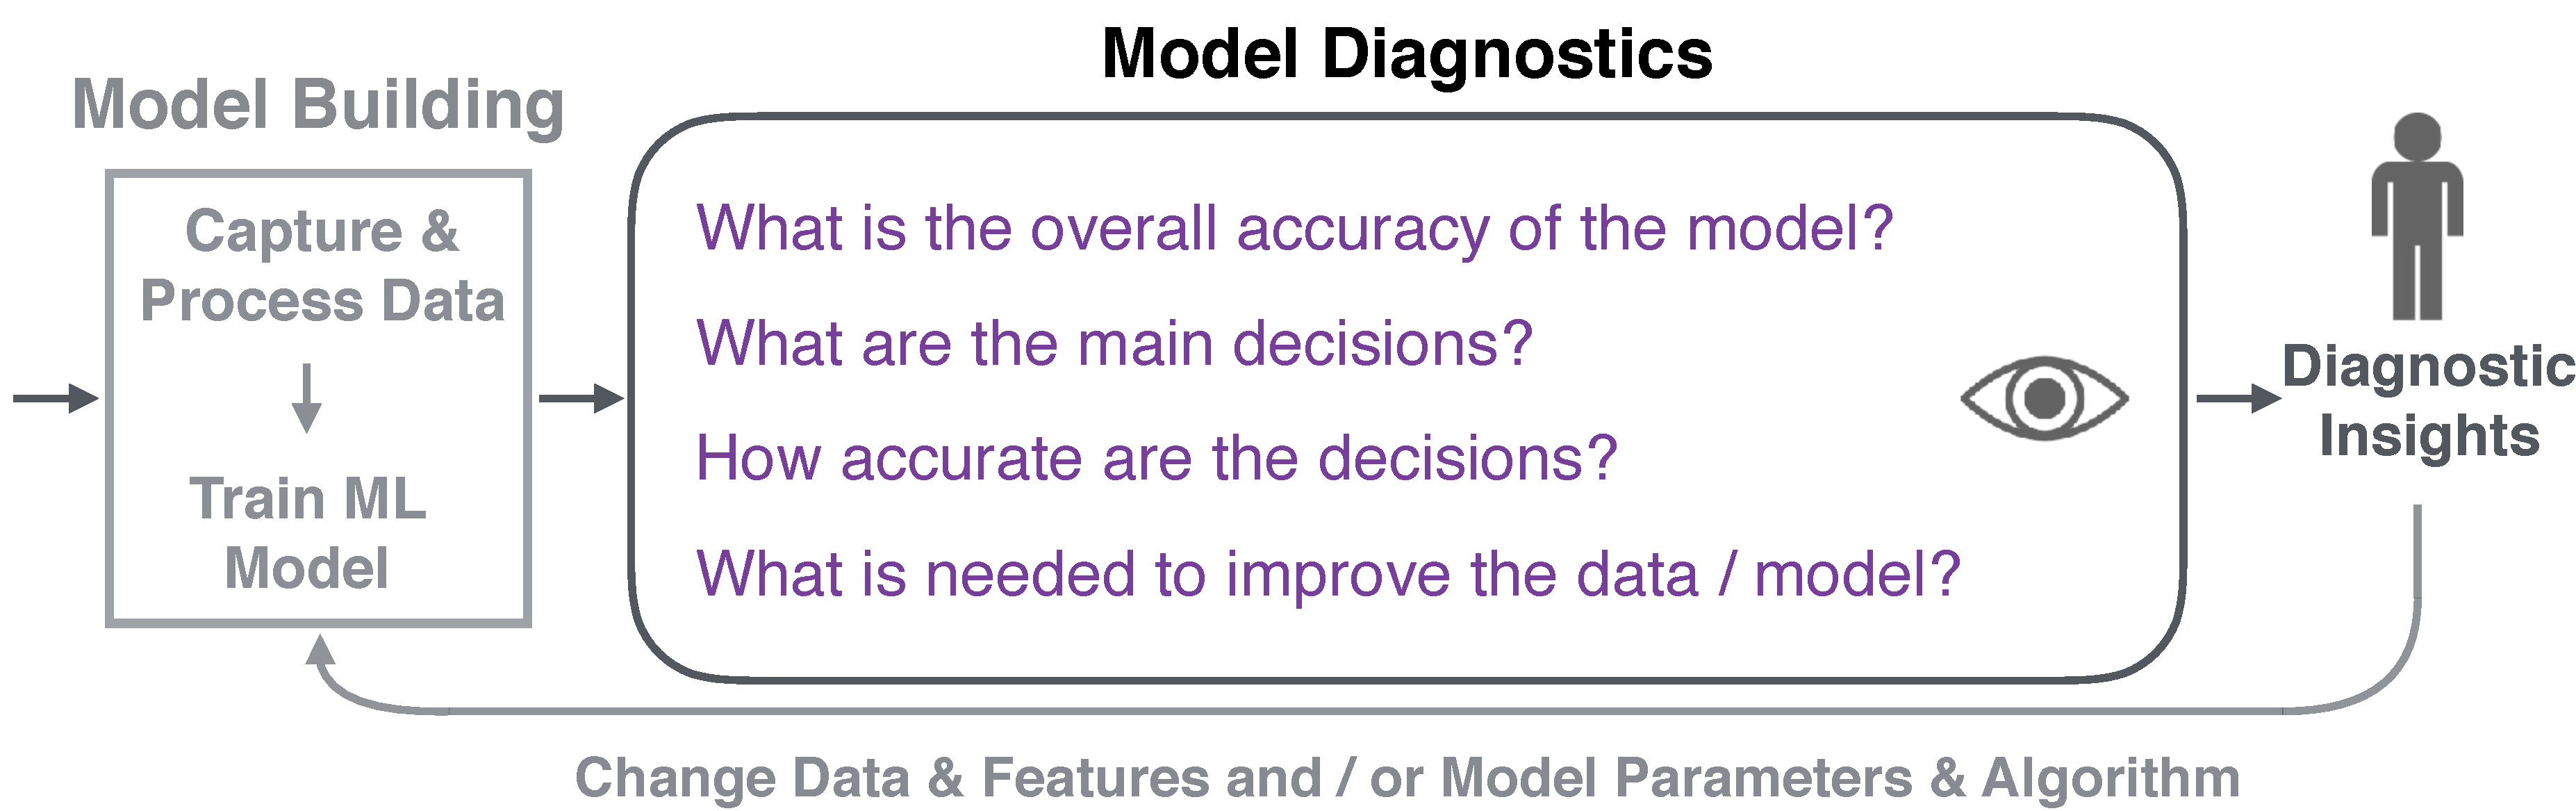
\includegraphics[width=\textwidth]{figs/workflow_large}
\caption[The model diagnostic workflow.]{
The proposed \textit{model diagnostic} workflow extends the conventional \textit{model building} workflow in machine learning for enabling domain experts to reason about the semantic validity of the decisions made by any model through multiple linked visualizations.
This ultimately helps to improve data acquisition and model generation processes belonging to the original workflow.
}
\label{figs:workflow_intro}
\end{figure}

\subsection{Model Diagnostic Workflow}
In the third stage, we overcome those limitations by leveraging \emph{instance-level explanations}. Instance-level explanations are defined as the smallest change, to an instance vector, necessary to change the predicted outcome label. Aggregating over those explanations and statistically analyzing the resulting instance subsets, proves as powerful novel approach for understanding the behavior of a model. Additionally, we propose a Model Diagnostic workflow (see \figref{figs:workflow_intro}) that helps identify flaws in the \emph{input data}, used to train and test the model.

\begin{table}[t]
     \begin{tabular}{l|c|c|c} 
     \textbf{Approach} & \makebox[0pt][l]{\textbf{Instances}}\phantom{Aggregated} & \textbf{Aggregated} & \makebox[0pt][l]{\textbf{Global}}\phantom{Aggregated} \\ 
     \hline
     \hline
     \infuse & & & X \Tstrut\\
     \hline
     \prospector & X & & X \Tstrut\\
     \hline
     \textit{Model Diagnostic workflow} & & X & \Tstrut\\
    \end{tabular}
    \centering
    \caption[Locality of decision analyses of the presented approaches.]{Locality of decision analyses of the presented approaches. \textbf{Instances} refers to analyzing decisions for one instance at a time. \textbf{Aggregated} refers to analyzing decisions for groups of instances and \textbf{Global} refers to analyzing decisions globally without inspecting decisions for individual instances.}
    \label{tab:locality}
\end{table}

We use this workflow to analyze a predictive modeling problem revolving around patient admission to a hospital, of patients in the emergency department of said hospital. Accurately predicting whether a patient eventually gets admitted to the hospital helps reducing costs. The major limiting factor of this prediction task is the need for input features readily, and electronically, available at the earliest point possible. To this extend we initially used features of prescribed medications as this information is immediately available electronically. Our analysis showed that there are clear groups of patients where the predictive model is very helpful. However, there are some groups of patients where it is impossible for the predictive model to make accurate predictions given the provided information. One of those groups is patients receiving Diatrizoate Meglumine, a contrast medium for CAT or PET scans. This medication only indicates that a scan was performed, but does not carry information about the result of the scan. However, the result of the scan is the deciding factor whether a patient needs further care or can get sent home. Thus, with the given information it is impossible for the predictive model to make a decision that performs better than random guessing. Including more information in the form of additional features does indeed help with this problem but pushes the time when a decision can be made further back. One possible solution is to utilize the predictive model only for the confident groups of patients and wait for the doctors' decisions in other cases. This example illustrates that it is not only possible to \textbf{understand decision making} of a predictive model through the \textbf{Model Diagnostic workflow} based on \textbf{aggregated instance-level explanations}, but also how it can be applied for \textbf{semantic validation} and \textbf{feature engineering} on the input data.

\subsection{User Study on Aggregating Explanations}
In order to show the generalizability of the Model Diagnostic Workflow we conducted a user study to explore the effectiveness of aggregated instance-level explanations in detecting biases in the input data.

First, we generalized aggregating instance-level explanations to numerical input data.
We achieved this by using histograms of the input features, similar to \cite{seekaview}, ordered by the features' aggregated importance.
Furthermore, we allowed the comparison of selected, meaningful, subsets to each other.
Then, we compared this aggregated representation, in a user study, to the commonly used approach of individually inspecting instance-level explanations one-by-one using a tabular representation.

We found that aggregating instance-level explanations, with our method, significantly \textbf{outperforms} inspecting \textbf{individual explanations} in its ability to enable detection of biases in the data.
However, our method \textbf{requires explanations} in order to perform correctly.
Additionally, we found that instance-level explanations \textbf{hurt} bias detection performance for a \textbf{tabular representation}.
We hypothesize that the added difficulty of inspecting a table without the help of explanations forces users to \textbf{interact} more strongly with the user interface, thus providing better results.
This is a known effect (see Hullman~\etal~\cite{6064986}).

All in all, aggregating instance-level explanations perform as well as explanation-free tabular representations, which require high user engagement.
Additionally, our method promises a higher scalability due to its independence from the total number of instances.

Furthermore, we could reproduce findings from Stumpf~\etal~\cite{harmful}, claiming that instance-level explanations might make users over-confident in their understanding of a model.
However, we also showed that aggregated instance-level explanations overcome this problem.

% In addition to those promising results, there is still work to do.
% It still needs to be shown that the proposed workflow of statistical analysis of instance-level explanations can be successfully applied to other data types than binary feature vectors, such as numerical features or highly redundant features such as found in images.
% Early results in this direction indicate that it might be beneficial to abandon the focus on features to explain machine learning models, but rather focus on instances directly.
% That is using instance-level explanations to obtain groups of \emph{instances} with similar behavior and then visualize those groups (\eg, using techniques proposed by \cite{seekaview}) in order to \emph{implicitly} explain them.
% This provides more flexible explanations than those proposed earlier as their capability goes beyond ``Feature A and feature B positively impact the prediction for this group of instances" to also allow insights of the form ``The number of circles formed by black pixels contribute positively to the prediction" which would be very difficult to formulate by a machine but are easily formulated by humans using visualizations.
% Furthermore, we are going to run a study on the implications on confidence in and trust of machine learning models when using different explanation approaches.
% \todo{END?}